
\documentclass{article}

\usepackage{ amssymb }
\usepackage{ mathrsfs }
\usepackage{graphicx}

\setlength\parindent{0pt} % Removes all indentation from paragraphs


\begin{document}
\title{Physics Problems: \#2}

\author{For Lucas}

\date{\today}
\maketitle


\section*{Cylinders Tower$^1$}

Consider a infinitely tall system of identical massive cylinders and massless planks shown in \ref{fig:tower}. The moment of inertia of each cylinder is $I = \frac{MR^2}{2}$. There are two cylinders at each level and the number of levels is infinite. The cylinders do not slip with respect to the planks, but the bottom plank is free to slide on a table. If you pull on the bottom plank so that it accelerates horizontally with acceleration $a$, \textit{what is the horizontal acceleration of the bottom row of cylinders?}.\\

\begin{figure}[h!]
\begin{center}
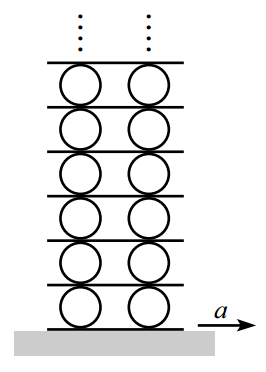
\includegraphics[width=0.3\textwidth]{tower.png}
\end{center}
\caption{Cylinder Tower.}
\label{fig:tower}
\end{figure}


\vspace{2mm}

\begin{center}
\noindent\rule{8cm}{0.4pt}\\
\end{center}

\noindent [1] \texttt{https://www.physics.harvard.edu/academics/undergrad/problems}

\end{document}